\makeatletter
\def\input@path{{../../}}
\makeatother
\documentclass[../../main.tex]{subfiles}
\graphicspath{
	{../../img/}
	{../img/}
	{img/}
}

\begin{document}

\begin{examples}

\;

\begin{enumerate}
\item Рассмотрим
\begin{equation*}
    \begin{cases}
        z = 1 + iy,\\
        -1 \leq y \leq 1.
    \end{cases}
\end{equation*}
\begin{center}
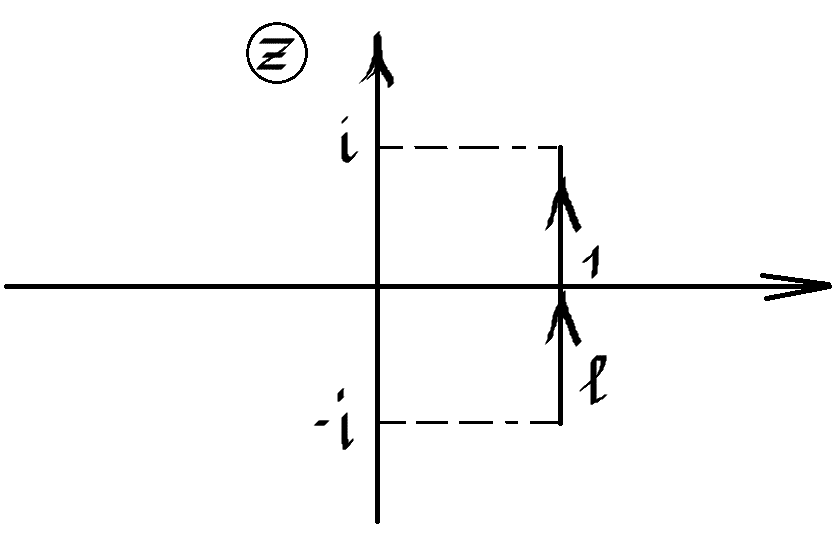
\includegraphics[height=0.3\textwidth]{lec30_1.png}
\end{center}

Рассмотрим образ $L$ этого отрезка при 
$w = z^2 = (x + iy)^2 = x^2 - y^2 + 2ixy$:
\begin{gather*}
    \begin{cases}
        u = \Re w = x^2 - y^2,\\
        v = \Im w = 2xy,
    \end{cases} \\
    L:
    \begin{cases}
        x = 1\\
        y\big|_{-1}^1
    \end{cases}
    \implies
    \begin{cases}
        u = 1 - y^2\\
        v = 2y\big|_{-2}^2
    \end{cases}
    \implies
    u = 1 - \frac{v^2}{4},\ v\big|_{-2}^2 
\end{gather*}

\begin{center}
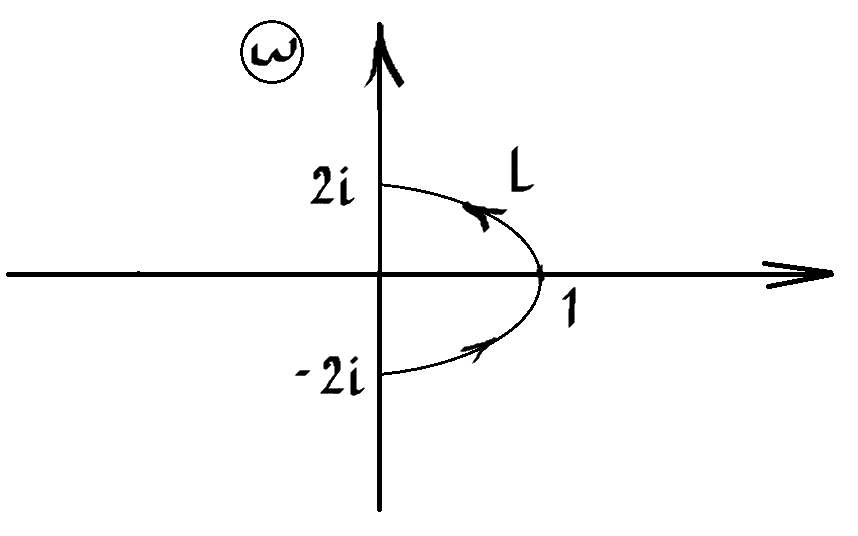
\includegraphics[height=0.3\textwidth]{lec30_2.png}
\end{center}

\[\begin{gathered}
\text{Длина }L \stackrel{\eqref{lec30:1}}{=}
\left[
     f'(z) = \left(z^2\right)' = 2z
\right]
= \int\limits_l{2\abs z \abs{dz}} = 
\left[
  z = 1 + iy,\ y|_{-1}^1
\right]
=\\=
\left[
  \begin{array}{ccc}
     |z| = \sqrt{1 + y^2}\\
     dz = idy \implies |dz| = dy
  \end{array}
\right]
= 2 \int\limits_{-1}^1{\sqrt{1 + y^2}\ dy} = 
4\int\limits_0^1{\sqrt{1 + y^2}\ dy} =\\= 2
\left[
  \sqrt{1 + y^2} + \ln(y + \sqrt{1 + y^2})
\right]_0^1 =
2(\sqrt{2} + \ln(1 + \sqrt{2})).
\end{gathered}\]

\item На комплексной плоскости рассмотрим квадрат $D$:
$\begin{cases}
    0 \leq x \leq 1,\\
    0 \leq y \leq 1;
\end{cases}$ \hspace{-1.1em} и отображение ${w = z^2}$.
\begin{center}
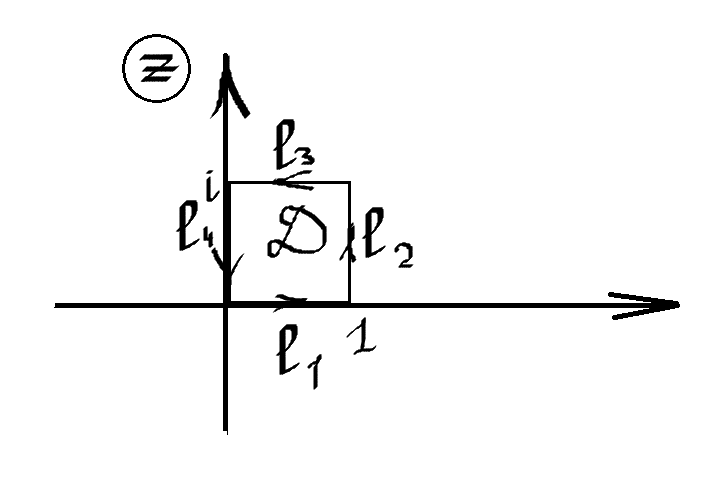
\includegraphics[height=0.3\textwidth]{lec30_3.png}
\end{center}
\[\begin{cases}
u = \Re w = \Re\ (x + iy)^2 = x^2 - y^2 \\
v = \Im w = \Im\ (x + iy)^2 = 2xy
\end{cases}\]

Рассмотрим все четыре стороны квадрата:
\begin{itemize}
\item[а)] $l_1: y = 0,\ 0 \leq x \leq 1 \stackrel{w}{\implies} L_1:
\begin{cases}
    u = x^2\big|_0^1\\
    v = 0
\end{cases}$
\begin{center}
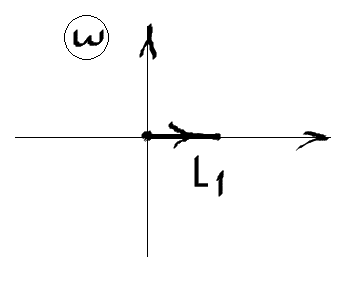
\includegraphics[height=0.3\textwidth]{lec30_4.png}
\end{center}

\item[б)]
$l_2: x = 1, 0 \leq x \leq 1 \stackrel{w}{\implies}
L_2: \begin{cases}
    u = 1 - y^2\\
    v = 2y\big|_0^2
\end{cases} \hspace{-1em} \iff
\begin{cases}
    u = 1 - \frac{v^2}{4}\\
    v\big|_0^2
\end{cases}$
\begin{center}
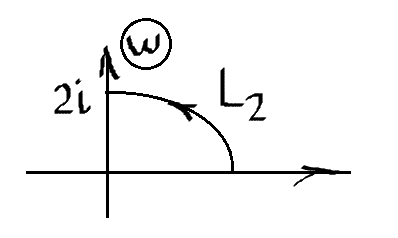
\includegraphics[height=0.3\textwidth]{lec30_5.png}
\end{center}

\item[в)]
$l_3: 
\begin{cases}
    y = 1\\
    x\big|_1^0
\end{cases} \hspace{-1em} \stackrel{w}{\implies}
L_3:
\begin{cases}
    u = x^2 - 1\\
    v = 2x\big|_2^0
\end{cases} \hspace{-1em} \iff
\begin{cases}
    u = \frac{v^2}{4} - 1\\
    v\big|_2^0
\end{cases}$
\begin{center}
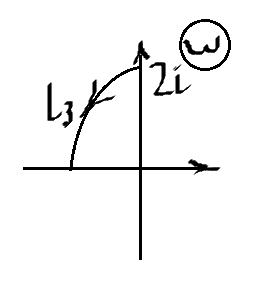
\includegraphics[height=0.3\textwidth]{lec30_6.png}
\end{center}

\item[г)]
$l_4:
\begin{cases}
    x = 0\\
    y\big|_1^0
\end{cases}
\hspace{-1em} \stackrel{w}{\implies}
L_4:
\begin{cases}
    u = -y^2\big|_1^0\\
    v = 0
\end{cases}$
\begin{center}
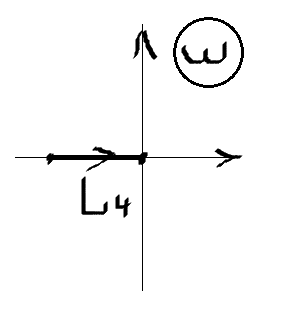
\includegraphics[height=0.3\textwidth]{lec30_7.png}
\end{center}
\end{itemize}

Имеем для $L$:

\begin{center}
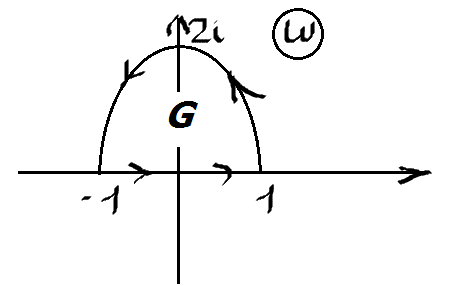
\includegraphics[height=0.3\textwidth]{lec30_8.png}
\end{center}
\[\begin{gathered}
\text{Площадь G} \stackrel{\eqref{lec30:2}}{=}  \left[
  f'(z) = 2z
\right]
= \iint\limits_D{|2z|^2dxdy} = 4\iint\limits_D{\left(x^2 + y^2\right)
dxdy} = \\ =
4\int\limits_0^1{dx}\int\limits_0^1{\left(x^2 + y^2\right) dy} = 
4\int\limits_0^1\left(x^2y + \frac{y^3}{3}\right)\bigg|_{y=0}^{y=1}\ dx = 
4\int\limits_0^1{\left(x^2 + \frac{1}{3}\right) dx} = 4\left(\frac{1}{3} +
\frac{1}{3}\right) = \frac{8}{3}.
\end{gathered}\]

\end{enumerate}
\end{examples}

\end{document}
